\section{Spark::Sp\-Glsl\-Manager Class Reference}
\label{classSpark_1_1SpGlslManager}\index{Spark::SpGlslManager@{Spark::SpGlslManager}}
{\tt \#include $<$Sp\-Glsl\-Manager.h$>$}

Collaboration diagram for Spark::Sp\-Glsl\-Manager:\begin{figure}[H]
\begin{center}
\leavevmode
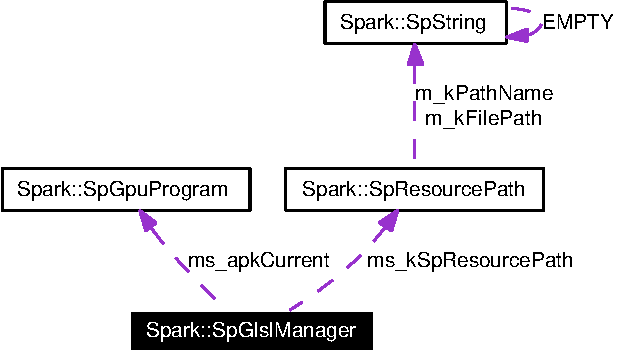
\includegraphics[width=166pt]{classSpark_1_1SpGlslManager__coll__graph}
\end{center}
\end{figure}


\subsection{Detailed Description}
Static manager class for interfacing with GLSL. 

Definition at line 38 of file Sp\-Glsl\-Manager.h.\subsection*{Public Member Functions}
\begin{CompactItemize}
\item 
{\bf $\sim$Sp\-Glsl\-Manager} ()
\begin{CompactList}\small\item\em Construction:. \item\end{CompactList}\end{CompactItemize}
\subsection*{Static Public Member Functions}
\begin{CompactItemize}
\item 
bool {\bf compile} ({\bf Sp\-Gpu\-Program} $\ast$pk\-Sp\-Gpu\-Program)
\begin{CompactList}\small\item\em Operations:. \item\end{CompactList}\item 
bool {\bf bind} ({\bf Sp\-Gpu\-Program} $\ast$pk\-Sp\-Gpu\-Program)
\item 
bool {\bf enable} ({\bf Sp\-Gpu\-Program} $\ast$pk\-Sp\-Gpu\-Program)
\item 
bool {\bf disable} ({\bf Sp\-Gpu\-Program} $\ast$pk\-Sp\-Gpu\-Program)
\item 
bool {\bf release} ({\bf Sp\-Gpu\-Program} $\ast$pk\-Sp\-Gpu\-Program)
\item 
bool {\bf is\-Supported} (const {\bf Sp\-Gpu\-Program} $\ast$pk\-Sp\-Gpu\-Program)
\item 
{\bf Sp\-Gpu\-Program} $\ast$ {\bf load\-From\-File} (const char $\ast$ac\-Filename, {\bf Sp\-Gpu\-Program::Type})
\item 
{\bf Sp\-Glsl\-Vertex\-Program} $\ast$ {\bf load\-Vertex\-Program\-From\-File} (const char $\ast$ac\-Filename)
\item 
{\bf Sp\-Glsl\-Fragment\-Program} $\ast$ {\bf load\-Fragment\-Program\-From\-File} (const char $\ast$ac\-Filename)
\item 
void {\bf print\-Info\-Log} (unsigned int ui\-Handle)
\item 
{\bf Sp\-Resource\-Path} \& {\bf searchpath} ()
\item 
void {\bf enable\-Texture\-Pass\-Through} (bool b\-Is\-Rectangle=false)
\item 
void {\bf enable\-Fragment\-Pass\-Through} ()
\item 
void {\bf enable\-Fragment\-Programs} ()
\item 
void {\bf enable\-Vertex\-Programs} ()
\item 
void {\bf disable\-Fragment\-Programs} ()
\item 
void {\bf disable\-Vertex\-Programs} ()
\end{CompactItemize}
\subsection*{Static Protected Attributes}
\begin{CompactItemize}
\item 
{\bf Sp\-Resource\-Path} {\bf ms\_\-k\-Sp\-Resource\-Path}
\begin{CompactList}\small\item\em Internal Data:. \item\end{CompactList}\item 
{\bf Sp\-Gpu\-Program} $\ast$ {\bf ms\_\-apk\-Current} [Sp\-Gpu\-Program::GPU\_\-PROGRAM\_\-COUNT]
\begin{CompactList}\small\item\em Static Data:. \item\end{CompactList}\end{CompactItemize}


\subsection{Constructor \& Destructor Documentation}
\index{Spark::SpGlslManager@{Spark::Sp\-Glsl\-Manager}!~SpGlslManager@{$\sim$SpGlslManager}}
\index{~SpGlslManager@{$\sim$SpGlslManager}!Spark::SpGlslManager@{Spark::Sp\-Glsl\-Manager}}
\subsubsection{\setlength{\rightskip}{0pt plus 5cm}Sp\-Glsl\-Manager::$\sim${\bf Sp\-Glsl\-Manager} ()}\label{classSpark_1_1SpGlslManager_a0}


Construction:. 

Definition at line 19 of file Sp\-Glsl\-Manager.cpp.

References ms\_\-apk\-Current, and release().

\subsection{Member Function Documentation}
\index{Spark::SpGlslManager@{Spark::Sp\-Glsl\-Manager}!bind@{bind}}
\index{bind@{bind}!Spark::SpGlslManager@{Spark::Sp\-Glsl\-Manager}}
\subsubsection{\setlength{\rightskip}{0pt plus 5cm}bool Sp\-Glsl\-Manager::bind ({\bf Sp\-Gpu\-Program} $\ast$ {\em pk\-Sp\-Gpu\-Program})\hspace{0.3cm}{\tt  [static]}}\label{classSpark_1_1SpGlslManager_e1}


Definition at line 112 of file Sp\-Glsl\-Manager.cpp.

References compile(), Spark::Sp\-Gpu\-Program::get\-Type(), Spark::Sp\-Gpu\-Program::get\-User\-Data(), and ms\_\-apk\-Current.

Referenced by Spark::Sp\-Vertex\-Noise\-Sb::initialize().\index{Spark::SpGlslManager@{Spark::Sp\-Glsl\-Manager}!compile@{compile}}
\index{compile@{compile}!Spark::SpGlslManager@{Spark::Sp\-Glsl\-Manager}}
\subsubsection{\setlength{\rightskip}{0pt plus 5cm}bool Sp\-Glsl\-Manager::compile ({\bf Sp\-Gpu\-Program} $\ast$ {\em pk\-Sp\-Gpu\-Program})\hspace{0.3cm}{\tt  [static]}}\label{classSpark_1_1SpGlslManager_e0}


Operations:. 

Definition at line 32 of file Sp\-Glsl\-Manager.cpp.

References Spark::Sp\-Gpu\-Program::get\-Length(), Spark::Sp\-Gpu\-Program::get\-Source(), Spark::Sp\-Gpu\-Program::get\-Type(), is\-Supported(), print\-Info\-Log(), and Spark::Sp\-Gpu\-Program::set\-User\-Data().

Referenced by bind(), enable(), Spark::Sp\-Vertex\-Noise\-Sb::initialize(), and Spark::Sp\-Turbulence\-Op::initialize().\index{Spark::SpGlslManager@{Spark::Sp\-Glsl\-Manager}!disable@{disable}}
\index{disable@{disable}!Spark::SpGlslManager@{Spark::Sp\-Glsl\-Manager}}
\subsubsection{\setlength{\rightskip}{0pt plus 5cm}bool Sp\-Glsl\-Manager::disable ({\bf Sp\-Gpu\-Program} $\ast$ {\em pk\-Sp\-Gpu\-Program})\hspace{0.3cm}{\tt  [static]}}\label{classSpark_1_1SpGlslManager_e3}


Definition at line 152 of file Sp\-Glsl\-Manager.cpp.

Referenced by Spark::Sp\-Vertex\-Noise\-Sb::disable(), and Spark::Sp\-Turbulence\-Op::update\-Output\-Stream().\index{Spark::SpGlslManager@{Spark::Sp\-Glsl\-Manager}!disableFragmentPrograms@{disableFragmentPrograms}}
\index{disableFragmentPrograms@{disableFragmentPrograms}!Spark::SpGlslManager@{Spark::Sp\-Glsl\-Manager}}
\subsubsection{\setlength{\rightskip}{0pt plus 5cm}void Sp\-Glsl\-Manager::disable\-Fragment\-Programs ()\hspace{0.3cm}{\tt  [static]}}\label{classSpark_1_1SpGlslManager_e15}


Definition at line 347 of file Sp\-Glsl\-Manager.cpp.\index{Spark::SpGlslManager@{Spark::Sp\-Glsl\-Manager}!disableVertexPrograms@{disableVertexPrograms}}
\index{disableVertexPrograms@{disableVertexPrograms}!Spark::SpGlslManager@{Spark::Sp\-Glsl\-Manager}}
\subsubsection{\setlength{\rightskip}{0pt plus 5cm}void Sp\-Glsl\-Manager::disable\-Vertex\-Programs ()\hspace{0.3cm}{\tt  [static]}}\label{classSpark_1_1SpGlslManager_e16}


Definition at line 352 of file Sp\-Glsl\-Manager.cpp.\index{Spark::SpGlslManager@{Spark::Sp\-Glsl\-Manager}!enable@{enable}}
\index{enable@{enable}!Spark::SpGlslManager@{Spark::Sp\-Glsl\-Manager}}
\subsubsection{\setlength{\rightskip}{0pt plus 5cm}bool Sp\-Glsl\-Manager::enable ({\bf Sp\-Gpu\-Program} $\ast$ {\em pk\-Sp\-Gpu\-Program})\hspace{0.3cm}{\tt  [static]}}\label{classSpark_1_1SpGlslManager_e2}


Definition at line 132 of file Sp\-Glsl\-Manager.cpp.

References compile(), Spark::Sp\-Gpu\-Program::get\-Type(), Spark::Sp\-Gpu\-Program::get\-User\-Data(), and ms\_\-apk\-Current.

Referenced by Spark::Sp\-Vertex\-Noise\-Sb::enable(), and Spark::Sp\-Turbulence\-Op::update\-Output\-Stream().\index{Spark::SpGlslManager@{Spark::Sp\-Glsl\-Manager}!enableFragmentPassThrough@{enableFragmentPassThrough}}
\index{enableFragmentPassThrough@{enableFragmentPassThrough}!Spark::SpGlslManager@{Spark::Sp\-Glsl\-Manager}}
\subsubsection{\setlength{\rightskip}{0pt plus 5cm}void Sp\-Glsl\-Manager::enable\-Fragment\-Pass\-Through ()\hspace{0.3cm}{\tt  [static]}}\label{classSpark_1_1SpGlslManager_e12}


Definition at line 308 of file Sp\-Glsl\-Manager.cpp.\index{Spark::SpGlslManager@{Spark::Sp\-Glsl\-Manager}!enableFragmentPrograms@{enableFragmentPrograms}}
\index{enableFragmentPrograms@{enableFragmentPrograms}!Spark::SpGlslManager@{Spark::Sp\-Glsl\-Manager}}
\subsubsection{\setlength{\rightskip}{0pt plus 5cm}void Sp\-Glsl\-Manager::enable\-Fragment\-Programs ()\hspace{0.3cm}{\tt  [static]}}\label{classSpark_1_1SpGlslManager_e13}


Definition at line 337 of file Sp\-Glsl\-Manager.cpp.\index{Spark::SpGlslManager@{Spark::Sp\-Glsl\-Manager}!enableTexturePassThrough@{enableTexturePassThrough}}
\index{enableTexturePassThrough@{enableTexturePassThrough}!Spark::SpGlslManager@{Spark::Sp\-Glsl\-Manager}}
\subsubsection{\setlength{\rightskip}{0pt plus 5cm}void Sp\-Glsl\-Manager::enable\-Texture\-Pass\-Through (bool {\em b\-Is\-Rectangle} = {\tt false})\hspace{0.3cm}{\tt  [static]}}\label{classSpark_1_1SpGlslManager_e11}


Definition at line 263 of file Sp\-Glsl\-Manager.cpp.\index{Spark::SpGlslManager@{Spark::Sp\-Glsl\-Manager}!enableVertexPrograms@{enableVertexPrograms}}
\index{enableVertexPrograms@{enableVertexPrograms}!Spark::SpGlslManager@{Spark::Sp\-Glsl\-Manager}}
\subsubsection{\setlength{\rightskip}{0pt plus 5cm}void Sp\-Glsl\-Manager::enable\-Vertex\-Programs ()\hspace{0.3cm}{\tt  [static]}}\label{classSpark_1_1SpGlslManager_e14}


Definition at line 342 of file Sp\-Glsl\-Manager.cpp.\index{Spark::SpGlslManager@{Spark::Sp\-Glsl\-Manager}!isSupported@{isSupported}}
\index{isSupported@{isSupported}!Spark::SpGlslManager@{Spark::Sp\-Glsl\-Manager}}
\subsubsection{\setlength{\rightskip}{0pt plus 5cm}bool Sp\-Glsl\-Manager::is\-Supported (const {\bf Sp\-Gpu\-Program} $\ast$ {\em pk\-Sp\-Gpu\-Program})\hspace{0.3cm}{\tt  [static]}}\label{classSpark_1_1SpGlslManager_e5}


Definition at line 176 of file Sp\-Glsl\-Manager.cpp.

References Spark::Sp\-Gpu\-Program::get\-Type().

Referenced by compile().\index{Spark::SpGlslManager@{Spark::Sp\-Glsl\-Manager}!loadFragmentProgramFromFile@{loadFragmentProgramFromFile}}
\index{loadFragmentProgramFromFile@{loadFragmentProgramFromFile}!Spark::SpGlslManager@{Spark::Sp\-Glsl\-Manager}}
\subsubsection{\setlength{\rightskip}{0pt plus 5cm}{\bf Sp\-Glsl\-Fragment\-Program} $\ast$ Sp\-Glsl\-Manager::load\-Fragment\-Program\-From\-File (const char $\ast$ {\em ac\-Filename})\hspace{0.3cm}{\tt  [static]}}\label{classSpark_1_1SpGlslManager_e8}


Definition at line 235 of file Sp\-Glsl\-Manager.cpp.

References Spark::Sp\-Resource\-Path::load\-Text\-File(), and searchpath().

Referenced by Spark::Sp\-Turbulence\-Op::initialize(), load\-From\-File(), and Spark::Sp\-Vertex\-Noise\-Sb::Sp\-Vertex\-Noise\-Sb().\index{Spark::SpGlslManager@{Spark::Sp\-Glsl\-Manager}!loadFromFile@{loadFromFile}}
\index{loadFromFile@{loadFromFile}!Spark::SpGlslManager@{Spark::Sp\-Glsl\-Manager}}
\subsubsection{\setlength{\rightskip}{0pt plus 5cm}{\bf Sp\-Gpu\-Program} $\ast$ Sp\-Glsl\-Manager::load\-From\-File (const char $\ast$ {\em ac\-Filename}, {\bf Sp\-Gpu\-Program::Type})\hspace{0.3cm}{\tt  [static]}}\label{classSpark_1_1SpGlslManager_e6}


Definition at line 212 of file Sp\-Glsl\-Manager.cpp.

References load\-Fragment\-Program\-From\-File(), and load\-Vertex\-Program\-From\-File().\index{Spark::SpGlslManager@{Spark::Sp\-Glsl\-Manager}!loadVertexProgramFromFile@{loadVertexProgramFromFile}}
\index{loadVertexProgramFromFile@{loadVertexProgramFromFile}!Spark::SpGlslManager@{Spark::Sp\-Glsl\-Manager}}
\subsubsection{\setlength{\rightskip}{0pt plus 5cm}{\bf Sp\-Glsl\-Vertex\-Program} $\ast$ Sp\-Glsl\-Manager::load\-Vertex\-Program\-From\-File (const char $\ast$ {\em ac\-Filename})\hspace{0.3cm}{\tt  [static]}}\label{classSpark_1_1SpGlslManager_e7}


Definition at line 223 of file Sp\-Glsl\-Manager.cpp.

References Spark::Sp\-Resource\-Path::load\-Text\-File(), and searchpath().

Referenced by Spark::Sp\-Turbulence\-Op::initialize(), load\-From\-File(), and Spark::Sp\-Vertex\-Noise\-Sb::Sp\-Vertex\-Noise\-Sb().\index{Spark::SpGlslManager@{Spark::Sp\-Glsl\-Manager}!printInfoLog@{printInfoLog}}
\index{printInfoLog@{printInfoLog}!Spark::SpGlslManager@{Spark::Sp\-Glsl\-Manager}}
\subsubsection{\setlength{\rightskip}{0pt plus 5cm}void Sp\-Glsl\-Manager::print\-Info\-Log (unsigned int {\em ui\-Handle})\hspace{0.3cm}{\tt  [static]}}\label{classSpark_1_1SpGlslManager_e9}


Definition at line 252 of file Sp\-Glsl\-Manager.cpp.

Referenced by compile().\index{Spark::SpGlslManager@{Spark::Sp\-Glsl\-Manager}!release@{release}}
\index{release@{release}!Spark::SpGlslManager@{Spark::Sp\-Glsl\-Manager}}
\subsubsection{\setlength{\rightskip}{0pt plus 5cm}bool Sp\-Glsl\-Manager::release ({\bf Sp\-Gpu\-Program} $\ast$ {\em pk\-Sp\-Gpu\-Program})\hspace{0.3cm}{\tt  [static]}}\label{classSpark_1_1SpGlslManager_e4}


Definition at line 158 of file Sp\-Glsl\-Manager.cpp.

References Spark::Sp\-Gpu\-Program::get\-User\-Data(), and Spark::Sp\-Gpu\-Program::set\-User\-Data().

Referenced by Spark::Sp\-Vertex\-Noise\-Sb::destroy(), and $\sim$Sp\-Glsl\-Manager().\index{Spark::SpGlslManager@{Spark::Sp\-Glsl\-Manager}!searchpath@{searchpath}}
\index{searchpath@{searchpath}!Spark::SpGlslManager@{Spark::Sp\-Glsl\-Manager}}
\subsubsection{\setlength{\rightskip}{0pt plus 5cm}{\bf Sp\-Resource\-Path} \& Sp\-Glsl\-Manager::searchpath ()\hspace{0.3cm}{\tt  [static]}}\label{classSpark_1_1SpGlslManager_e10}


Definition at line 247 of file Sp\-Glsl\-Manager.cpp.

References ms\_\-k\-Sp\-Resource\-Path.

Referenced by load\-Fragment\-Program\-From\-File(), and load\-Vertex\-Program\-From\-File().

\subsection{Member Data Documentation}
\index{Spark::SpGlslManager@{Spark::Sp\-Glsl\-Manager}!ms_apkCurrent@{ms\_\-apkCurrent}}
\index{ms_apkCurrent@{ms\_\-apkCurrent}!Spark::SpGlslManager@{Spark::Sp\-Glsl\-Manager}}
\subsubsection{\setlength{\rightskip}{0pt plus 5cm}{\bf Sp\-Gpu\-Program} $\ast$ {\bf Sp\-Glsl\-Manager::ms\_\-apk\-Current}\hspace{0.3cm}{\tt  [static, protected]}}\label{classSpark_1_1SpGlslManager_t1}


Static Data:. 

Definition at line 17 of file Sp\-Glsl\-Manager.cpp.

Referenced by bind(), enable(), and $\sim$Sp\-Glsl\-Manager().\index{Spark::SpGlslManager@{Spark::Sp\-Glsl\-Manager}!ms_kSpResourcePath@{ms\_\-kSpResourcePath}}
\index{ms_kSpResourcePath@{ms\_\-kSpResourcePath}!Spark::SpGlslManager@{Spark::Sp\-Glsl\-Manager}}
\subsubsection{\setlength{\rightskip}{0pt plus 5cm}{\bf Sp\-Resource\-Path} {\bf Sp\-Glsl\-Manager::ms\_\-k\-Sp\-Resource\-Path}\hspace{0.3cm}{\tt  [static, protected]}}\label{classSpark_1_1SpGlslManager_t0}


Internal Data:. 

Definition at line 16 of file Sp\-Glsl\-Manager.cpp.

Referenced by searchpath().

The documentation for this class was generated from the following files:\begin{CompactItemize}
\item 
{\bf Sp\-Glsl\-Manager.h}\item 
{\bf Sp\-Glsl\-Manager.cpp}\end{CompactItemize}
